\documentclass[aspectratio=169, xcolor=table]{beamer}

% Packages
\usepackage[utf8]{inputenc}
\usepackage{graphicx}
\usepackage{tikz}
\usepackage{booktabs}
\usepackage{hyperref}
\usepackage{xcolor}
\usepackage{multicol}

% Theme
\usetheme{Madrid}
\usecolortheme{whale}
\usefonttheme{professionalfonts}

% Custom Colors Strategy
\definecolor{DrishtiBlue}{RGB}{20, 50, 100}
\definecolor{DrishtiGold}{RGB}{200, 160, 50}
\setbeamercolor{structure}{fg=DrishtiBlue}
\setbeamercolor{frametitle}{bg=DrishtiBlue, fg=white}
\setbeamercolor{title}{bg=DrishtiBlue, fg=white}

% TikZ Libraries for Diagrams
\usetikzlibrary{shapes, arrows.meta, positioning, shadows, backgrounds}

% Title Slide Info
\title[InboxPilot]{InboxPilot: An Agentic AI Application}
\subtitle{Architecting Foundational Models into Autonomous Systems}
\author[Drishti IAS]{Drishti IAS}
\date{March 17, 2026}
\titlegraphic{
    
\begin{tikzpicture}
        \node[star, star points=7, star point ratio=0.8, fill=DrishtiGold, scale=0.5] {};
    \end{tikzpicture}
}

\begin{document}

% Slide 1: Title
\begin{frame}[plain]
    \titlepage
\end{frame}

% Slide 2: Table of Contents
\begin{frame}{Agenda}
    % Note: Run pdflatex twice for this to populate
    \tableofcontents
\end{frame}

% Section 1: Introduction
\section{1. Introduction to InboxPilot}

\begin{frame}{What is InboxPilot?}
    \begin{block}{Overview}
        \textbf{InboxPilot} is a specialized Agentic AI application designed to autonomously process, classify, and respond to incoming email and text streams using a distributed multi-agent system.
    \end{block}
    
    \vspace{0.3cm}
    \begin{columns}[T]
        \begin{column}{0.48\textwidth}
            \begin{block}{What It Does}
                \begin{itemize}
                    \item \textbf{Ingests:} Reads continuous data streams via tools (e.g., IMAP).
                    \item \textbf{Reasons:} Dynamically synthesizes context.
                    \item \textbf{Acts:} Calls external APIs to retrieve specific missing data.
                \end{itemize}
            \end{block}
        \end{column}
        
        \begin{column}{0.48\textwidth}
            \begin{block}{The Agents Involved}
                \begin{itemize}
                    \item \textbf{Classify Agent:} Detects user intent.
                    \item \textbf{Fetch Agent:} Searches and retrieves context.
                    \item \textbf{Respond Agent:} Generates final drafts.
                    \item \textbf{Supervisor:} Orchestrates routing logic.
                \end{itemize}
            \end{block}
        \end{column}
    \end{columns}
\end{frame}

\begin{frame}{The Core Artefacts}
    Our framework divides the ecosystem into four fundamental pillars, essential for any robust Agentic platform:
    \vspace{0.3cm}
    \begin{enumerate}
        \item \textbf{Models:} Foundational reasoning engines and schemas.
        \item \textbf{Tools:} Actionable capabilities connecting to the outside world.
        \item \textbf{Agents:} Specialized autonomous workers maintaining context.
        \item \textbf{Orchestration:} Directed logic governing overarching data flow.
    \end{enumerate}
\end{frame}

% Section 2: Artefacts
\section{2. Development Artefacts}

\begin{frame}{Artefact 1: Models}
    \textbf{Models form the brain of the platform.} We rely on standard abstractions loaded directly into the execution environment.
    
    \vspace{0.3cm}
    \begin{block}{Source Components}
        \begin{itemize}
            \item \texttt{config.yaml}: Static definitions for model hyperparameters.
            \item \texttt{inboxpilot/models.py}: Pydantic structures acting as exact schemas for validation.
            \item \texttt{inboxpilot/state.py}: The memory structure passed continuously during runtime.
        \end{itemize}
    \end{block}
    
    \vspace{0.2cm}
    \textbf{Runtime:} Loaded natively into the Python environment and injected as configuration context across all executing containers.
\end{frame}

\begin{frame}{Artefact 2: Tools}
    \textbf{Language models alone cannot act.} \textit{Tools} provide the APIs to enact change in the external world.
    
    \vspace{0.3cm}
    \begin{block}{Application Tools (\texttt{inboxpilot/tools/})}
        \begin{itemize}
            \item \texttt{calendar\_tool.py}: External calendar management.
            \item \texttt{imap\_tool.py}: Email stream ingestion.
            \item \texttt{search\_tool.py}: Open-world information retrieval.
        \end{itemize}
    \end{block}
    
    \vspace{0.2cm}
    \textbf{Runtime Integration:} Executed as live, parameter-driven functions operating securely within an Agent's isolated execution process.
\end{frame}

\begin{frame}{Artefact 3: Agents}
    \textbf{Agents are independent micro-nodes of intelligence.} Each agent in InboxPilot is bounded to a specific persona and logic flow.
    
    \vspace{0.3cm}
    \begin{block}{The Workforce}
        \begin{itemize}
            \item \textbf{Classify Agent:} Determines user intent from the raw input payload.
            \item \textbf{Fetch Agent:} Retrieves required context via dynamic tool usage.
            \item \textbf{Respond Agent:} Formulates the final synthesized output.
        \end{itemize}
    \end{block}
    
    \vspace{0.2cm}
    \textbf{Microservices:} Deployed as live ASGI microservices. Each agent has its own \texttt{Dockerfile} (e.g., \texttt{services/classify-service/Dockerfile}) to guarantee clean, scalable bounds.
\end{frame}

\begin{frame}{Artefact 4: Orchestration}
    \textbf{If Agents are the workers, Orchestration is the manager.} It handles complex interactions across the distributed system.
    
    \vspace{0.3cm}
    \begin{block}{Components}
        \begin{itemize}
            \item \textbf{Supervisor Node (\texttt{services/supervisor/}):} Houses \texttt{graph.py}, dynamically routing logic between the workforce.
            \item \textbf{Communication (\texttt{a2a/}):} Agent-to-Agent message passing protocol over the internal network.
            \item \textbf{Infrastructure (\texttt{docker-compose.yml}):} Links the master orchestrator to its subordinate agents.
        \end{itemize}
    \end{block}
\end{frame}

% Section 3: Architecture
\section{3. System Architecture \& LangGraph Diagram}

\begin{frame}{System Architecture \& DAG Routing}
    \centering
    \resizebox{0.9\textwidth}{!}{%
    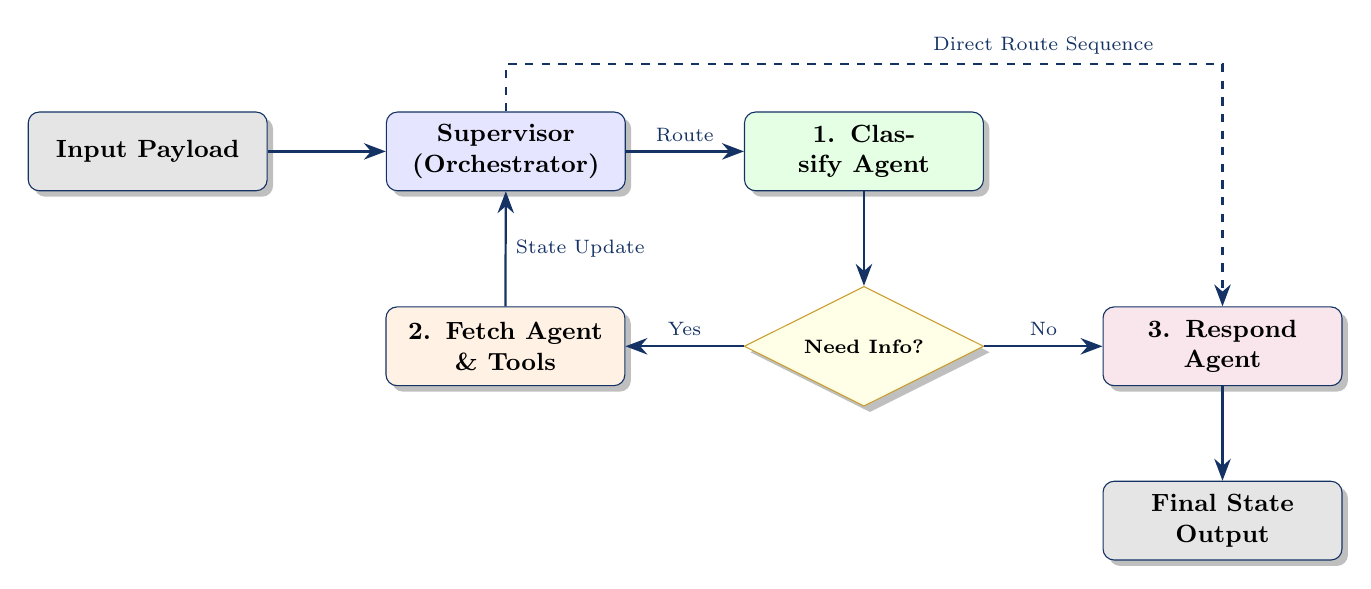
\begin{tikzpicture}[
        node distance=1.2cm and 1.5cm,
        box/.style={rectangle, draw=DrishtiBlue, fill=blue!10, text width=2.8cm, align=center, rounded corners, drop shadow, minimum height=1cm, font=\small\bfseries},
        arrow/.style={-{Stealth[scale=1.2]}, thick, DrishtiBlue},
        decision/.style={diamond, aspect=2, draw=DrishtiGold, fill=yellow!10, text width=2cm, align=center, drop shadow, font=\scriptsize\bfseries}
    ]
        
        % Nodes
        \node[box, fill=gray!20] (input) {Input Payload};
        \node[box, right=of input] (supervisor) {Supervisor \\ (Orchestrator)};
        \node[box, fill=green!10, right=of supervisor] (classify) {1. Classify Agent};
        \node[decision, below=of classify] (needinfo) {Need Info?};
        \node[box, fill=orange!10, left=of needinfo] (fetch) {2. Fetch Agent \\ \& Tools};
        \node[box, fill=purple!10, right=of needinfo] (respond) {3. Respond Agent};
        \node[box, fill=gray!20, below=of respond] (output) {Final State Output};
        
        % Connections
        \draw[arrow] (input) -- (supervisor);
        \draw[arrow] (supervisor) -- (classify) node[midway, above, font=\scriptsize] {Route};
        \draw[arrow] (classify) -- (needinfo);
        \draw[arrow] (needinfo) -- (fetch) node[midway, above, font=\scriptsize] {Yes};
        \draw[arrow] (fetch.north) -- (supervisor.south) node[midway, right, font=\scriptsize] {State Update};
        \draw[arrow] (needinfo) -- (respond) node[midway, above, font=\scriptsize] {No};
        \draw[arrow] (respond) -- (output);
        \draw[arrow, dashed] (supervisor.north) |- ([yshift=0.6cm]classify.north) -| (respond.north) node[pos=0.25, above, font=\scriptsize] {Direct Route Sequence};
        
    \end{tikzpicture}%
    }
    
    \vspace{0.4cm}
    \scriptsize \textit{Dynamic LangGraph Execution: The Orchestrator routes data and maintains the overarching state memory.}
\end{frame}

% Section 4: Conclusion
\section{4. Conclusion}

\begin{frame}{Conclusion \& Summary of Achievements}
    \begin{itemize}
        \item \textbf{Separation of Concerns:} Rigidly partitioned Models, Tools, Agents, and Orchestration logic.
        \item \textbf{Scalability:} Containerized components into a distributed microservice web via Docker.
        \item \textbf{Autonomy:} Established an event-driven reasoning system capable of dynamic routing and state persistence.
    \end{itemize}
    
    \vspace{0.5cm}
    \begin{block}{Looking Forward}
        Establishing \textbf{InboxPilot} as a foundational reference architecture for future enterprise-grade, multi-agent platforms.
    \end{block}
\end{frame}

\begin{frame}[plain]
    \centering
    \vspace{2cm}
    \Huge \textbf{Thank You}
    
    \vspace{1cm}
    \Large \textbf{Questions?}
\end{frame}

\end{document}
